%% 1. DUAL-DISPLAY NOTES:
%\documentclass[hyperref={bookmarks=false}]{beamer}
%\usepackage{pgfpages}
%\setbeameroption{show notes on second screen=left}

% 2. NOTES ON SEPARATE SLIDES:
%\documentclass[xcolor=dvipsnames,9pt,show notes]{beamer}

% 3. NOTES ONLY:
%\documentclass[xcolor=dvipsnames,9pt,show only notes]{beamer}

% 4. HANDOUTS:
%\documentclass[xcolor=dvipsnames,9pt,handout,show notes]{beamer}

% 5. NO NOTES: ONLY ONE THAT BUILDS WITHOUT WARNINGS
\documentclass[xcolor=dvipsnames,9pt,hide notes,mathserif]{beamer}
%\setbeameroption{show only notes}
%\setbeameroption{show notes}
\usepackage{enumerate,amsmath,amssymb,fancyhdr,mathrsfs,amsthm,url,stmaryrd}
\usepackage{pgfpages}
\usepackage{listings}

%% For creating a handout:
%\pgfpagesuselayout{4 on 1}[border shrink=5mm]
%\mode<handout>{\setbeamercolor{background canvas}{bg=black!5}}

\setbeamerfont{structure}{family=\rmfamily,shape=\scshape} 
\usepackage{graphicx}
\usepackage{tikz}
\usepackage{scalefnt}
\usetikzlibrary{matrix,arrows}

\usepackage{mathrsfs,textcomp}
\setbeamertemplate{navigation symbols}{}
\usepackage{verbatim}
\usepackage[mathcal]{euscript}

\definecolor{Crimson}{rgb}{0.800,0.000,0.200}
\definecolor{darkred}{rgb}{0.5,0,0}
\newcommand{\Alert}[1]{\textcolor{darkred}{{\bf \emph{#1}}}}
\renewcommand{\alert}[1]{\textcolor{darkred}{\emph{#1}}}

\setbeamercolor{block title example}{fg=darkred,bg=white} %orange!20!black}

\usecolortheme[named=darkred]{structure} 
\setbeamertemplate{items}[ball] 
\setbeamertemplate{blocks}[rounded][shadow=true] 

\mode<presentation>{\usetheme{boxes}}

\usepackage[english]{babel}
\usepackage[latin1]{inputenc}
\usepackage{times}
\usepackage[T1]{fontenc}
% Or whatever. Note that the encoding and the font should match. If T1
% does not look nice, try deleting the line with the fontenc.

\title[Synchronizing Automata]{Synchronizing Automata\\
{\small and}\\
The \v{C}ern\'{y} Conjecture}
\author[William DeMeo]{William DeMeo\\
{\small \url{williamdemeo@gmail.com}}
}
\institute[\url{williamdemeo@gmail}]{{\small {\color{darkred}  University of South Carolina}}}

\date[CU Graduate Algebra Seminar]{
Graduate Algebra Seminar\\
 University of Colorado\\[6pt]
April 11, 2013
}

\subject{Universal Algebra; Lattice Theory.}% (optional) inserted into PDF info catalog.

% TOC pops up at the beginning of each subsection:
\AtBeginSubsection[]{
  \begin{frame}<beamer>
    \frametitle{Outline}
    \tableofcontents[currentsection,currentsubsection]
  \end{frame}
}

\setbeamercovered{opaque}

%%%% INSERT MACROS %%%%
\newcommand{\bA}{\ensuremath{\mathbf{A}}}
\newcommand{\cA}{\ensuremath{\mathcal{A}}}
\newcommand{\fA}{\ensuremath{\mathfrak{A}}}
\newcommand{\sA}{\ensuremath{\mathscr{A}}}

\newcommand{\cB}{\ensuremath{\mathcal{B}}}
\newcommand{\bB}{\ensuremath{\mathbf{B}}}
\newcommand{\bBi}{\ensuremath{\mathbf{B}_i}}
\newcommand{\sB}{\ensuremath{\mathscr{B}}}
\newcommand{\fB}{\ensuremath{\mathfrak{B}}}

\newcommand{\bF}{\ensuremath{\mathbf{F}}}
\newcommand{\sF}{\ensuremath{\mathcal{F}}}

\newtheorem{prop}[theorem]{Proposition}
\newtheorem{assumption}[theorem]{Assumption}
\theoremstyle{definition}
\newtheorem{question}[theorem]{Question}
\newcounter{claim}
\newtheorem{claim}[claim]{Claim}
\newcounter{conjecture}
\newtheorem{conjecture}[conjecture]{Conjecture}
\newtheorem{case}{Case}
\theoremstyle{remark}
\newtheorem*{computations}{Computations}
\newtheorem*{remark}{Remark}
\newtheorem*{remarks}{Remarks}
\newtheorem*{notation}{Notation}
\numberwithin{theorem}{section}
\numberwithin{claim}{section}
\numberwithin{equation}{section}
\numberwithin{conjecture}{section}

\newcommand{\czerny}{\v{C}ern\'{y}}
\newcommand{\defn}[1]{\textcolor{darkred}{\textit{#1}}}
\newcommand{\IE}{{\small IE}}
\newcommand{\Op}{\ensuremath{\operatorname{Op}}}

\newcommand{\<}{\ensuremath{\langle}}
\renewcommand{\>}{\ensuremath{\rangle}}
\newcommand{\Clo}{\ensuremath{\mathrm{Clo}}}




%%%%%%%%%%%%  BEGIN DOCUMENT %%%%%%%%%%%%%%%

\begin{document}
\thicklines


%%% START HERE %%%
\frame[label=titlepage]{
  \titlepage
\vskip-3mm
  \begin{columns}
    \begin{column}{0.8\textwidth}
      \begin{center}
        {\small {\it These slides and other resources are available at}}\\[4pt]
 {\color{darkred}       \url{http://williamdemeo.wordpress.com}}
         \end{center}
       \end{column}
    \end{columns}
}

\providecommand{\url}[1]{{#1}}
\providecommand{\urlprefix}{URL }


\section{Introduction}

%%% SLIDE 1 %%%
\begin{frame}[label=intro]{Synchronizing automata}
A \Alert{finite automaton} is a triple $\bA = \<Q, \Sigma,
\delta\>$ where
\begin{itemize}
\item $Q$ is a set of \alert{states}
\item $\Sigma$ is a set of \alert{letters} (the \emph{input alphabet})
\item $\delta: Q\times \Sigma \rightarrow Q$ is a \alert{transition function}
\end{itemize}

\vskip2mm

\uncover<2->{If $\bA$ is currently in state $q\in Q$, then upon input $a\in \Sigma$
 the next state is $\delta(q,a)$.  }

\vskip2mm

\uncover<3->{Given an input sequence of letters  $a_0, a_1, \dots, a_{n-1}$, the resulting state is
\begin{equation}
  \label{eq:1}
\delta(\cdots \delta(\delta(q,a_{0}),a_{1})\cdots,a_{n-1})
\end{equation}
}
\uncover<4->{If we write $aq$ in place of $\delta(q,a)$, then~(\ref{eq:1}) is simply
$a_{n-1}a_{n-2} \dots a_1a_{0}q$.}

\vskip2mm

\uncover<5->{Let $\Sigma^*$ denote the free monoid obtained by composing letters.  

\vskip2mm

A \alert{word} $w\in \Sigma^*$ is just a string of letters, 
$w = a_0 a_1 \dots a_{n-1}$, which 
acts on a state $q \in Q$ as you expect:
\[
wq = a_0 a_1 \dots a_{n-1}q
\]
}
\end{frame}

\begin{frame}[label=intro]{Synchronizing automata}
Viewed this way, the automaton $\<Q, \Sigma, \delta\>$ is simply a unary
algebra $\bA =\<Q, \Sigma\>$ with universe $Q$ and basic operations $\Sigma$.

\vskip2mm

\uncover<2->{$\bA$ is called \alert{synchronizing} if there exists a constant word
in $\Sigma^*$; \\that is, a term operation $w$ such that $wx = wy$ for all $x,
y \in Q$.

\vskip 2mm

Such $w$ are called \alert{reset words} for $\bA$.}

\vskip2mm

\uncover<3->{
  \begin{example}
  \begin{center}
        \begin{tikzpicture}[->,>=stealth',shorten >=1pt,auto,node distance=2cm,
          thick,main node/.style={circle,fill=blue!20,draw,font=\sffamily\small\bfseries},scale=.5]
          \draw[draw=none,font=\small] (-5,5) node {$Q = \{0, 1, 2, 3\}$};
 
         \alt<5->{\draw[draw=none,font=\small] (-5,4) node[red] {$a = (1, 1, 2, 3)$};}
          {\draw[draw=none,font=\small] (-5,4) node {$a = (1, 1, 2, 3)$};}

          \draw[draw=none,font=\small] (-5,3) node {$b = (1, 2, 3, 0)$};

          \uncover<4->{
            \draw[draw=none,font=\small] (-5,2) node {$\bA = \<Q, \{a, b\}\>$};
            \alt<5->{  \node[main node] (0) {0};
  \node[main node] (1) [right of=0] {1};
  \node[main node] (3) [above of=0] {3};
  \node[main node] (2) [right of=3] {2};

  \path[every node/.style={font=\sffamily\small}]
    (0) edge node [above] {$b$} (1)
        edge [red,bend right] node[below] [black]{$a$} (1)
    (1) edge node [right] {$b$} (2)
        edge [red,loop right] node [black]{$a$} (1)
    (2) edge node [above] {$b$} (3)
        edge [red,loop above] node [black]{$a$} (2)
    (3) edge node [right] {$b$} (0)
        edge [red,loop above] node [black]{$a$} (3);

%\draw[draw=none,font=\Large] (-3,5) node {$\mathscr{C}_4$};}{  \node[main node] (0) {0};
  \node[main node] (1) [right of=0] {1};
  \node[main node] (3) [above of=0] {3};
  \node[main node] (2) [right of=3] {2};

  \path[every node/.style={font=\sffamily\small}]
    (0) edge node [above] {$a,b$} (1)
        edge [bend right] node[below]{$a$} (1)
    (1) edge node [right] {$b$} (2)
        edge [loop right] node {$a$} (1)
    (2) edge node [above] {$b$} (3)
        edge [loop above] node {$a$} (2)
    (3) edge node [right] {$b$} (0)
        edge [loop above] node {$a$} (3);

%\draw[draw=none,font=\Large] (-3,5) node {$\mathscr{C}_4$};}
          }

          \uncover<6->{\draw[draw=none] (8,3) node {reset word:} (8,2) node {$abbbabbba$};}

        \end{tikzpicture}
    \end{center}
  \end{example}
}
\end{frame}

\begin{frame}[label=intro]{Synchronizing automata}

The notion was formalized in 1964 in a paper by Jan
\czerny, though implicitly it had been around since at
least 1956.

\vskip2mm

The idea of synchronization is natural and of
obvious importance: we aim to restore control over a
device whose current state is unknown.


\vskip2mm

For example, our view of an orbiting 
satellite may be temporarily obstructed by the Moon; 
once it comes back into view, we regain control and reorient it\\
(\czerny 's original motivation). 
\end{frame}

\newcommand{\widget}{(-1.5,-1.5)--(1.5,-1.5)--(1.5,1.5) -- (.5,1.5) -- (.5,2.25) -- (-.5,2.25) -- (-.5,1.5) -- (-1.5,1.5) -- (-1.5,-1.5)}
\begin{frame}[label=intro]{Synchronizing automata}
In the 80's, the notion was reinvented by engineers
working in a branch of robotics which deals with part
handling problems in industrial automation.

\vskip2mm

\uncover<2->{Suppose that one of the parts of a certain device has
the following shape:

\begin{center}
\begin{tikzpicture}[scale=.4]
  \draw \widget;
\end{tikzpicture}
\end{center}

Such parts will move along a conveyor belt and must be sorted and oriented before
assembly.}

\vskip2mm

\uncover<3->{Assume that only four initial orientations are possible, namely,
\begin{center}
\begin{tikzpicture}[scale=.4]
  \draw \widget;
  \draw[rotate=90,shift={(0cm,5cm)}] \widget;
  \draw[rotate=180,shift={(10cm,0cm)}] \widget;
  \draw[rotate=270,shift={(0cm,5cm)}] \widget;
  \node[circle,fill=blue!20,draw,font=\sffamily\small\bfseries] at (-10cm,0) {0};
  \node[circle,fill=blue!20,draw,font=\sffamily\small\bfseries] at (-5cm,0) {1};
  \node[circle,fill=blue!20,draw,font=\sffamily\small\bfseries] at (0,0) {2};
  \node[circle,fill=blue!20,draw,font=\sffamily\small\bfseries] at (5cm,0) {3};
\end{tikzpicture}
\end{center}
}
\end{frame}

\begin{frame}[label=intro]{Synchronizing automata}
  
\begin{center}
\begin{tikzpicture}[scale=.4]
  \draw \widget;
  \draw[darkred,rotate=90,shift={(0cm,5cm)}] \widget;
  \draw[rotate=180,shift={(10cm,0cm)}] \widget;
  \draw[rotate=270,shift={(0cm,5cm)}] \widget;
  \node[circle,fill=blue!20,draw,font=\sffamily\small\bfseries] at (-10cm,0) {0};
  \node[circle,fill=blue!20,draw,font=\sffamily\small\bfseries] at (-5cm,0) {1};
  \node[circle,fill=blue!20,draw,font=\sffamily\small\bfseries] at (0,0) {2};
  \node[circle,fill=blue!20,draw,font=\sffamily\small\bfseries] at (5cm,0) {3};
\end{tikzpicture}
\end{center}
\vskip2mm

Prior to assembly the part must be in position
{\bf 1}, \alert{``bump-left''} orientation.

\vskip2mm

{\bf Problem:} construct an orienter that
will put the part in bump-left position
independently of its initial orientation.

\end{frame}

\begin{frame}[label=intro]{Synchronizing automata}
  
{\bf Solution:} position two types of obstacles, short and tall, in the
path of the part.  When the
part passes a tall obstacle, it always rotates 90\textdegree.  When it passes a short
obstacle, it rotates by 90\textdegree\ iff it is in bump-down orientation. 

\begin{center}
\begin{tikzpicture}[scale=.4]
\uncover<1>{\draw \widget;}
\uncover<2>{\draw[shift={(2cm,0cm)}] \widget;}
\uncover<3>{\draw[shift={(3cm,0cm)}] \widget;}
\uncover<4>{\draw[rotate=-45,shift={(3cm,3.8cm)}] \widget;}
\uncover<5>{\draw[rotate=-90,shift={(-0.5cm,8cm)}] \widget;}
\uncover<1-5>{\draw[semithick] (5.3,-4)--(5.3,-1);}

\uncover<6>{\draw[rotate=-90] \widget;}
\uncover<7>{\draw[rotate=-90,shift={(0,2cm)}] \widget;}
\uncover<8>{\draw[rotate=-90,shift={(0,4cm)}] \widget;}
\uncover<9>{\draw[rotate=-90,shift={(0,6cm)}] \widget;}
\uncover<10>{\draw[rotate=-90,shift={(0,8cm)}] \widget;}
\uncover<6-10>{\draw[semithick,red] (5.3,-4)--(5.3,-2);}

\uncover<11>{\draw[rotate=-90] \widget;}
\uncover<12>{\draw[rotate=-90,shift={(0,2cm)}] \widget;}
\uncover<13>{\draw[rotate=-90,shift={(0,3cm)}] \widget;}
\uncover<14>{\draw[rotate=-135,shift={(-3.8,3cm)}] \widget;}
\uncover<15>{\draw[rotate=-180,shift={(-8cm,-.5)}] \widget;}
\uncover<11-15>{ \draw[semithick] (5.3,-4)--(5.3,-1);}

\uncover<16>{\draw[rotate=180] \widget;}
\uncover<17>{\draw[rotate=180,shift={(-2cm,0)}] \widget;}
\uncover<18>{\draw[rotate=180,shift={(-3cm,0)}] \widget;}
\uncover<19>{\draw[rotate=180,shift={(-4cm,0)}] \widget;}
\uncover<20>{\draw[rotate=135,shift={(-4.7cm,-4.4cm)}] \widget;}
\uncover<21>{\draw[rotate=90,shift={(-0.5cm,-8cm)}] \widget;}
\uncover<16-21>{\draw[semithick,red] (5.3,-4)--(5.3,-2);}

\uncover<22->{
  \draw \widget;
  \draw[rotate=90,shift={(0cm,5cm)}] \widget;
  \draw[rotate=180,shift={(10cm,0cm)}] \widget;
  \draw[rotate=270,shift={(0cm,5cm)}] \widget;
  \node[circle,fill=blue!20,draw,font=\sffamily\small\bfseries] at (-10cm,0) {0};
  \node[circle,fill=blue!20,draw,font=\sffamily\small\bfseries] at (-5cm,0) {1};
  \node[circle,fill=blue!20,draw,font=\sffamily\small\bfseries] at (0,0) {2};
  \node[circle,fill=blue!20,draw,font=\sffamily\small\bfseries] at (5cm,0) {3};
  \draw[semithick,red] (5.3,-4)--(5.3,-2);
  \draw (5.3,-4.5) node {$a$};
  \draw[semithick] (7.3,-4)--(7.3,-1);
  \draw (7.3,-4.5) node {$b$};
}
\end{tikzpicture}
\uncover<22->{
\begin{tikzpicture}[->,>=stealth',shorten >=1pt,auto,node distance=2cm,
  thick,main node/.style={circle,fill=blue!20,draw,font=\sffamily\small\bfseries},scale=.4]
    \node[main node] (0) {0};
  \node[main node] (1) [right of=0] {1};
  \node[main node] (3) [above of=0] {3};
  \node[main node] (2) [right of=3] {2};

  \path[every node/.style={font=\sffamily\small}]
    (0) edge node [above] {$b$} (1)
        edge [red,bend right] node[below] [black]{$a$} (1)
    (1) edge node [right] {$b$} (2)
        edge [red,loop right] node [black]{$a$} (1)
    (2) edge node [above] {$b$} (3)
        edge [red,loop above] node [black]{$a$} (2)
    (3) edge node [right] {$b$} (0)
        edge [red,loop above] node [black]{$a$} (3);

%\draw[draw=none,font=\Large] (-3,5) node {$\mathscr{C}_4$};
         % \uncover<6->{\draw[draw=none] (8,3) node {reset word:} (8,2) node {$abbbabbba$};}
\end{tikzpicture}
}
\end{center}

\end{frame}


\begin{frame}[shrink=10,label=CzernyFamily]{\v{C}ern\'{y}'s infinite family}
  \begin{columns}
    \begin{column}{0.5\textwidth}
      \begin{tikzpicture}[->,>=stealth',shorten >=1pt,auto,node distance=2cm,
        thick,main node/.style={circle,fill=blue!20,draw,font=\sffamily\small\bfseries},scale=.4]
          \node[main node] (2) {2};
  \node[main node] (0) [below left of=2] {0};
  \node[main node] (1) [below right of=2] {1};

  \path[every node/.style={font=\sffamily\small}]
    (0) edge node [above] {$a, b$} (1)
%        edge [bend right] node[below] {$a$} (1)
    (1) edge node [right] {$b$} (2)
        edge [loop right] node {$a$} (1)
    (2) edge node [left] {$b$} (0)
        edge [loop above] node {$a$} (2);

\draw[draw=none,font=\Large] (-3.5,2) node {$\mathscr{C}_3$};
        \uncover<2->{\draw[draw=none] (-4.5,0) node {reset word:}
          (-4.5,-1) node {$abba$};}
      \end{tikzpicture}
    \end{column}
    
    \begin{column}{0.5\textwidth}
      \uncover<3->{
        \begin{tikzpicture}[->,>=stealth',shorten >=1pt,auto,node distance=2cm,
          thick,main node/.style={circle,fill=blue!20,draw,font=\sffamily\small\bfseries},scale=.4]
            \node[main node] (0) {0};
  \node[main node] (1) [right of=0] {1};
  \node[main node] (3) [above of=0] {3};
  \node[main node] (2) [right of=3] {2};

  \path[every node/.style={font=\sffamily\small}]
    (0) edge node [above] {$a,b$} (1)
    (1) edge node [right] {$b$} (2)
        edge [loop right] node {$a$} (1)
    (2) edge node [above] {$b$} (3)
        edge [loop above] node {$a$} (2)
    (3) edge node [right] {$b$} (0)
        edge [loop above] node {$a$} (3);

%\draw[draw=none,font=\Large] (-3,5) node {$\mathscr{C}_4$};
          \draw[draw=none,font=\Large] (-3,5) node {$\mathscr{C}_4$};
          \uncover<4->{\draw[draw=none] (-4.5,3) node {reset word:}
            (-4.5,2) node {$abbbabbba$};}
        \end{tikzpicture}}
    \end{column}
    \end{columns}

    \begin{center}
      \uncover<5->{
        \begin{tikzpicture}[->,>=stealth',shorten >=1pt,auto,node distance=3cm,
          thick,main node/.style={circle,fill=blue!20,draw,font=\sffamily\small\bfseries},scale=.4]
            \node[main node] (0) at (0,8) {0};
  \node[main node] (1) at (3.25,6.5) {1};
  \node[main node] (2) at (6,4) {2};
  \node (3) at (7,1) {};
  \node (nm3) at (-7,1) {};
  \node[main node] (nm2) at (-6,4) {n-2};
  \node[main node] (nm1) at (-3.25,6.5) {n-1};

  \path[every node/.style={font=\sffamily\small}]
    (0) edge node [pos=.2]{$a,b$} (1)
    (1) edge node [left] {$b$} (2)
        edge [loop right] node {$a$} (1)
    (2) edge node [left] {$b$} (3)
        edge [loop right] node {$a$} (2)
    (nm3) edge node [right] {$b$} (nm2)
    (nm2) edge node [below] {$b$} (nm1)
        edge [loop left] node {$a$} (nm2)
    (nm1) edge node [below] {$b$} (0)
        edge [loop left] node {$a$} (nm1);

\draw[draw=none] (7,1) node {$\vdots$} (-7,1) node {$\vdots$};
\draw[draw=none,font=\Large] (-4,10) node {$\mathscr{C}_n$};
          \uncover<6->{\draw[draw=none] (-5,-1) node {reset word:}
            (3.2,-1) node {$abbb\cdots b abbb\cdots ba = (ab^{n-1})^{n-2}a$};}
          \uncover<7->{\draw[draw=none] (0,-2.5) node {length: $n(n-2)+1 = (n-1)^2$};}
        \end{tikzpicture}}
    \end{center}

\end{frame}

\begin{frame}[label=CzernyBound]{The \czerny\ bound}
  \begin{itemize}
  \item 
A synchronizing automaton with $n$ states \alert{reaches the
\czerny\ bound} if the minimum length of all reset words
is $(n-1)^2$. 

\vskip7mm

\item We present all known proper
synchronizing automata  with $n>2$ states.
\vskip7mm

{\small (``proper'' means removal of any letter results in a nonsynchronizing automaton)}
  \end{itemize}
\end{frame}


\begin{frame}[label=Sporadic]{Sporadic Examples}

There are three sporadic examples on 3 states:
\begin{center}
  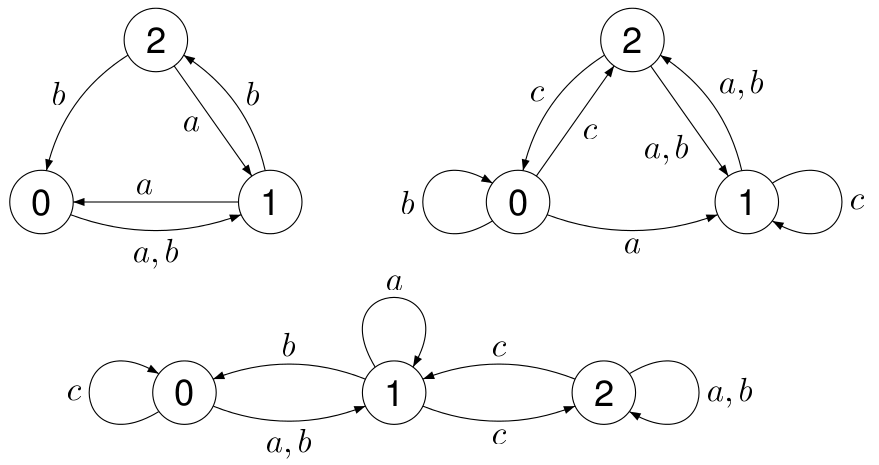
\includegraphics[height=2.25in]{Sporadic3}
\end{center}
\end{frame}

\begin{frame}[label=Sporadic]{Sporadic Examples}

For 4 states, three sporadic examples are known:
\begin{center}
  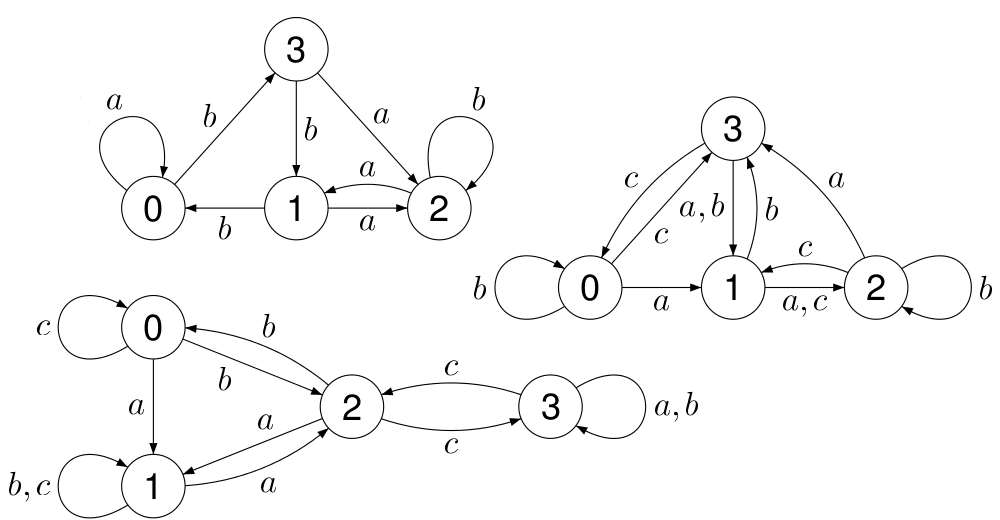
\includegraphics[height=2.25in]{Sporadic4}
\end{center}
\end{frame}

\begin{frame}[label=Sporadic]{Roman's Example}

For 5 states, a synchronizing automaton reaching the \czerny\ bound was
discovered by Adam Roman:
\begin{center}
  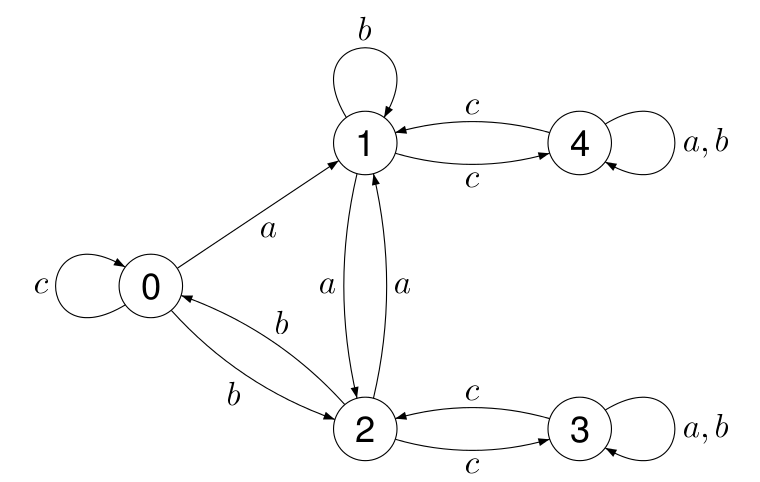
\includegraphics[height=2in]{Roman5}
\end{center}
\end{frame}


\begin{frame}[label=Sporadic]{Kari's Example}
The last in our list and the most remarkable example
was published in 2001 by Jarkko Kari. % (EATCS Bull., 73, 146).
\begin{center}
  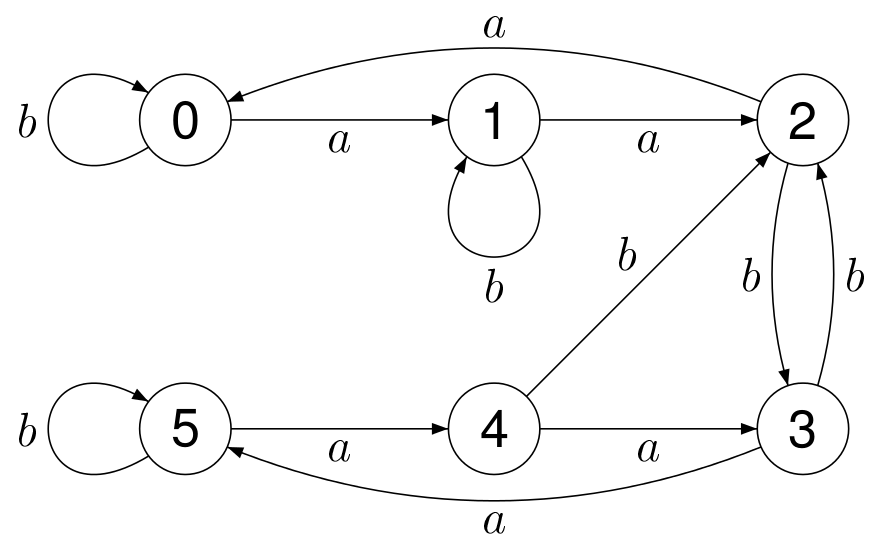
\includegraphics[height=1.5in]{Kari6}
\end{center}
\uncover<2->{Minimum length reset word: 
$a\,b\, b\,a\,b \,a\,b\, b\,a\,b\, b\,a\,b \, a\, a\,b\, b\,a\,b\, a\,b\, a\,b\,b\,a$}
\end{frame}

\begin{frame}[shrink=5,label=Clones]{Clones}{a brief review}
  \begin{itemize}
  \item<1->
For nonempty set $A$, let $\Op(A)$ be the set of all operations on $A$.
That is,
\[
\Op(A)  = \bigcup_{n<\omega} A^{(A^n)}
\]

\vskip2mm

  \item<2->
For each $k \leq n < \omega$, the $k$th \emph{projection operation} is
\[
p_k^n(x_1, \dots, x_n) = x_k
\]

\vskip2mm

  \item<2->
If $f\in A^{(A^n)}$ and $g_1, \dots, g_n \in A^{(A^k)}$, then a \emph{generalized
composition} is
\[
f[g_1, \dots, g_n]: (x_1, \dots, x_k) \mapsto f(g_1(x_1,\dots, x_k), \dots,
g_n(x_1,\dots, x_k))
\]

\vskip2mm

  \item<3->
A \alert{clone} on $A$ is a subset of $\Op(A)$ that contains all
projections and is closed under generalized compositions.

\vskip2mm

  \item<4->
Given $F \subseteq \Op(A)$, let $\Clo^A(F)$ denote the smallest clone on $A$
containing $F$.

\vskip2mm

  \item<4->
Let $\Clo_n^A(F)$ denote the $n$-ary members of $\Clo^A(F)$.

  \end{itemize}
\end{frame}


\begin{frame}[shrink=7,label=Clones]{Clones}{a brief review}
  \begin{itemize}
  \item<1->
If $\bA = \<A, F\>$ is an algebra, then $\Clo^A(F)$ is called the \alert{clone
  of term operations on} $\bA$, which we denote by $\Clo(\bA)$.

\end{itemize}
\uncover<2->{
\begin{theorem}
  
    Given $\bA$ and $n\in \omega$, the set $\Clo_n(\bA)$ is
    a subuniverse of the direct power algebra $\bA^{(A^n)}$.  It is generated by
    the projections $\{p_1^n, p_2^n, \dots, p_n^n\}$.

~
\end{theorem}

}
 \vskip3mm
\uncover<3->{
(Note that $\Clo_1(\bA)$ is the subuniverse of $\bA^A$ generated by $p_1^1$, the identity
 map.)
}
 \vskip3mm

\uncover<4->{
  \begin{example}
\[
A = \{0, 1, 2\} \qquad a = (1, 1, 2) \qquad b = (1,2,0)
\qquad \bA = \<A, \{a,b\}\>
\]

 \vskip2mm
\uncover<5->{
\hskip1cm $\Clo_1(\bA)$ is the subuniverse of $\bA^A = \bA \times \bA \times \bA$
generated by $(0,1,2)$.

~
}

\end{example}
}
\end{frame}

\newcommand{\bT}{\ensuremath{\mathbf{T}}}
\newcommand{\TX}{\ensuremath{T_\rho(X)}}
\newcommand{\TXn}{\ensuremath{T_\rho(X_n)}}
\newcommand{\bTX}{\ensuremath{\bT_{\rho}(X)}}
\newcommand{\bTXn}{\ensuremath{\bT_{\rho}(X_n)}}
\newcommand{\salg}{\ensuremath{\mathscr{A}_{\rho}}}
\begin{frame}[label=Terms]{Terms}{a brief review}
  \begin{itemize}
  \item<1->
 Let $\sF$ be a set of operation symbols and let 
$\rho : \sF \rightarrow \omega$
be a similarity type.

\vskip3mm

\item<1->
Let $F_n = \{ f\in \sF \mid \rho(f) = n\}$
  be the set of $n$-ary operation symbols in $\sF$.

\vskip3mm

\item<2-> Let $X$ be a set, disjoint from $\sF$, whose elements we call
  \emph{variables}.  

\vskip3mm

\item<2->
A \alert{word on the alphabet}
  $X\cup \sF$ is a finite string $a_1a_2\cdots a_{n}$, where $a_i\in X\cup \sF$. 
The \alert{product} of words is defined by concatenation.

\vskip3mm

\item<3-> The set $T_\rho(X)$ of \alert{terms of type} $\rho$ \alert{over} $X$
  is the smallest set $T$ of  words on the alphabet $X\cup \sF$ such that 
  \begin{itemize}
  \item $X\cup F_0 \subseteq T$
  \item If $t_1, \dots, t_{n} \in T$ and $f\in F_n$, then 
    $ft_1t_2\cdots t_{n} \in T$.
  \end{itemize}

\vskip3mm

  \item<3-> If $t_1, \dots, t_{n}$ are terms and $f\in F_n$ is an $n$-ary
    operation symbol, we often write $f(t_1,t_2,\cdots, t_{n})$ instead
    of $ft_1t_2\cdots t_{n}$.


\end{itemize}
\end{frame}

\begin{frame}[label=Terms]{Terms}{a brief review}
  \begin{itemize}
  \item<1->
For each $f\in F_n$ let
    $f^{\bTX}$ be the $n$-ary operation on $\TX$ that maps $(t_1, \dots, t_n)$
    to $ft_1 \dots t_n$.  

\vskip3mm

  \item<1-> 
Define \alert{term algebra of type} $\rho$ as follows
\[
\bTX = \< \TX, \{f^{\bTX} : f\in \sF\}\>
\]

\vskip1mm

    $\bTX$ is free in $\salg$ over $X$.

\vskip3mm

   \item<2-> Let $X_n = \{x_1, \dots, x_n\}$.
     For $t(x_1, \dots, x_n) \in \TXn$ and $\bA$ an algebra of type $\rho$,
     define an $n$-ary operation $t^\bA$ on $A$ by recursion on the ``height''
     of $t$:
\vskip3mm
-- if $t$ is the variable $x_i$ then $t^\bA(a_1, \dots, a_n) = a_i$
\vskip3mm
-- if $t=fs_1s_2\dots s_k$ where $f\in F_k$ and $s_1, \dots, s_k$ are
       terms, then 
       \[
       t^{\bA}(a_1, \dots, a_n) = f^{\bA}(s_1^{\bA}(a_1, \dots, a_n), \dots,
       s_k^{\bA}(a_1, \dots, a_n))
       \]

\end{itemize}
\end{frame}

\begin{frame}[label=ClonesAndTerms]{Connecting clones and terms}

Consider the map $\phi: X_n \rightarrow A^{(A^n)}$ defined by $\phi(x_i) = p_i^n$.

\vskip 2mm

\uncover<2->{
By freeness of $\bTXn$, there exists a unique hom $\bar{\phi} : \bTXn
   \rightarrow \bA^{(A^n)}$ extending $\phi$. 
}
\vskip 2mm

\uncover<2->{
 ...and for any $t\in \TXn$, we have
   $\bar{\phi}(t) = t^\bA$ (induct on height of $t$)
}
\vskip2mm

\uncover<3->{
  \begin{theorem}%[see, e.g., Bergman, p. 100]
\[
  \Clo_n(\bA) = \{t^\bA : t\in \TXn\}
\]

~
  \end{theorem}

\vskip2mm

{\it Proof:}  
For the unique hom above, we have $\bar{\phi}(t) = t^\bA \in \Clo_n(\bA)$.

\vskip1mm

~\phantom{Proof} The image $\bar{\phi}(\TXn)$ contains all the projections.
\vskip1mm

~\phantom{Proof} The projections generate the algebra $\mathbf{Clo}_n(\bA)$, so
\[\bar{\phi}(\TXn) =  \Clo_n(\bA)\]
}
\end{frame}

\begin{frame}[label=ClonesAndTerms]{Connecting clones and terms}
...and finally, we recall that if 
$\bF_\bA(X_n)$ denotes a free algebra in $V(\bA)$ with free generating set $X_n$, then
\[
\bF_\bA(X_n) \cong \bTXn / \Theta
\]
where two terms are equivalent mod $\Theta$ when they induce the same term
operation on every member of $V(\bA)$.  

\vskip2mm

Thus, taking $\Theta$ to be the kernel of $\bar{\phi}$, we have
$\bF_\bA(X_n) \cong \Clo_n(\bA)$.
\end{frame}

\begin{frame}
  
  \begin{example}
\[
A = \{0, 1, 2\} \qquad a = (1, 1, 2) \qquad b = (1,2,0)
\qquad \bA = \<A, \{a,b\}\>
\]

 \vskip2mm
\hskip1cm $\Clo_1(\bA)$ is the subuniverse of $\bA^A = \bA \times \bA \times \bA$
generated by $(0,1,2)$
 \vskip2mm
\[
\Clo_1(\bA)\cong \bF_\bA\{(0,1,2)\}
\]

~
\end{example}

\end{frame}

\begin{frame}[shrink=16,label=FreeAlgebraExample]{}
\begin{figure}[h!]
  \centering
{\scalefont{.3}
  \begin{tikzpicture}[->,>=stealth',shorten >=1pt,auto,node distance=2cm,
thick, main node/.style={circle,fill=blue!20,draw,font=\sffamily\small},scale=.3]
% Main triangle

%  \node[main node] (012) at (20,20) {012};
  \node (012) at (20,20) [circle,fill=gray!20,draw,font=\sffamily\small]{012};
  \node[main node] (120) [above right of=012] {120};
  \node[main node] (201) [above left of=012] {201};

  \path[every node/.style={font=\sffamily\small}]
    (012) edge node [below] {$b$} (120)
    (120) edge node [above] {$b$} (201)
    (201) edge node [below] {$b$} (012);

% first middle triangle
  \node[main node] (112) at (18,15) {112};
  \node[main node] (001) [below left of=112] {001};
  \node[main node] (220) [below of=112] {220};

  \path[every node/.style={font=\sffamily\small}]
    (001) edge node [left] {$b$} (112)
    (112) edge node [right] {$b$} (220)
    (220) edge node [below] {$b$} (001);

% second middle triangle
  \node[main node] (002) at (22,15) {002};
  \node[main node] (221) [below of=002] {221};
  \node[main node] (110) [below right of=002] {110};

  \path[every node/.style={font=\sffamily\small}]
    (221) edge node [left] {$b$} (002)
    (002) edge node [above] {$b$} (110)
    (110) edge node [below] {$b$} (221)

    (220) edge [red] node [below,black] {$a$} (221)
    (002) edge [red] node [above,black] {$a$} (112);


% first right hand triangle
  \node[main node] (121) at (33,20) {121};
  \node[main node] (010) [below left of=121] {010};
  \node[main node] (202) [below of=121] {202};

  \path[every node/.style={font=\sffamily\small}]
    (010) edge node [left] {$b$} (121)
    (121) edge node [right] {$b$} (202)
    (202) edge node [below] {$b$} (010);

% second right hand triangle
  \node[main node] (020) at (37,20) {020};
  \node[main node] (212) [below of=020] {212};
  \node[main node] (101) [below right of=020] {101};

  \path[every node/.style={font=\sffamily\small}]
    (212) edge node [left] {$b$} (020)
    (020) edge node [above] {$b$} (101)
    (101) edge node [below] {$b$} (212)

    (202) edge [red] node [below,black] {$a$} (212)
    (020) edge [red] node [above,black] {$a$} (121)

    (012) edge [red] node [right,black] {$a$} (112)
    (120) edge [red] node [above,black] {$a$} (121);

% first left hand triangle
  \node[main node] (211) at (7,20) {211};
  \node[main node] (022) [below of=211] {022};
  \node[main node] (100) [below right of=211] {100};

  \path[every node/.style={font=\sffamily\small}]
    (211) edge node [left] {$b$} (022)
    (022) edge node [below] {$b$} (100)
    (100) edge node [below] {$b$} (211);

% second left hand triangle
  \node[main node] (200) at (3,20) {200};
  \node[main node] (122) [below of=200] {122};
  \node[main node] (011) [below left of=200] {011};

  \path[every node/.style={font=\sffamily\small}]
    (200) edge node [above] {$b$} (011)
    (011) edge node [above] {$b$} (122)
    (122) edge node [right] {$b$} (200)

    (022) edge [red] node [below,black] {$a$} (122)
    (200) edge [red] node [above,black] {$a$} (211)

    (201) edge [red] node [right,black] {$a$} (211);


% Bottom triangle
  \node[main node] (111) at (20,0) {111};
  \node[main node] (000) [below right of=111] {000};
  \node[main node] (222) [below left of=111] {222};

  \path[every node/.style={font=\sffamily\small}]
    (000) edge node [left] {$b$} (111)
    (111) edge node [above] {$b$} (222)
    (222) edge node [below] {$b$} (000)

    (000) edge [red,bend right] node [right,black] {$a$} (111)

    (011) edge [red,bend right] node [left,black] {$a$} (111)
    (100) edge [red,bend right] node [left,black] {$a$} (111)
    (001) edge [red] node [left,black] {$a$} (111)
    (110) edge [red] node [right,black] {$a$} (111)
    (010) edge [red,bend left] node [right,black] {$a$} (111)
    (101) edge [red,bend left] node [right,black] {$a$} (111);

% LOOPS
  \path[every node/.style={font=\sffamily\small}]
    (211) edge [red,loop above]  (211)
    (122) edge [red,loop below]  (122)
    (212) edge [red,loop below]  (212)
    (221) edge [red,loop below]  (221)
    (121) edge [red,loop above]  (121)
    (111) edge [red,loop below]  (111)
    (222) edge [red,loop left]  (222)
    (112) edge [red,loop left]  (112);

\draw[draw=none,font=\small] (2.5,4) node {$A = \{0, 1, 2\}$};
\draw[draw=none,font=\small] (2.5,2) node {$a = (1, 1, 2)$};
\draw[draw=none,font=\small] (2.5,0) node {$b = (1, 2, 0)$};
\draw[draw=none,font=\small] (2.5,-2) node {$\bA = \<A, \{a, b\}\>$};
\draw[draw=none,font=\small] (2.5,-4) node {$\bF_{\bA}\{(0,1,2)\} \leq \bA^A$};
%\draw[draw=none,font=\small] (2.5,4) node {$A = \{0, 1, 2\}$};
\draw[draw=none,font=\small] (2.5,2) node[red] {$a = (1, 1, 2)$};
\draw[draw=none,font=\small] (2.5,0) node {$b = (1, 2, 0)$};
\draw[draw=none,font=\small] (2.5,-2) node {$\bA = \<A, \{a, b\}\>$};
\draw[draw=none,font=\small] (2.5,-4) node {$\bF_{\bA}\{(0,1,2)\} \leq \bA^A$};
%\draw[draw=none,font=\small] (2.5,-6) node {$|F_{\bA}| =24 \quad |A^A| = 27$};


\end{tikzpicture}
}
\end{figure}
\end{frame}

\begin{frame}[shrink=16,label=FreeAlgebraExamplePath]{}
\begin{figure}[h!]
  \centering
{\scalefont{.3}
\only<1>{
\begin{tikzpicture}[->,>=stealth',shorten >=1pt,auto,node distance=2cm,
thick, main node/.style={circle,fill=blue!20,draw,font=\sffamily\small},scale=.3]
% Main triangle

%  \node[main node] (012) at (20,20) {012};
  \node (012) at (20,20) [circle,fill=gray!20,draw,font=\sffamily\small]{012};
  \node[main node] (120) [above right of=012] {120};
  \node[main node] (201) [above left of=012] {201};

  \path[every node/.style={font=\sffamily\small}]
    (012) edge  (120)
    (012) edge  (120)
    (120) edge  (201)
    (201) edge  (012);

% first middle triangle
  \node[main node] (112) at (18,15) {112};
%  [circle,fill=green!20,draw,font=\sffamily\small] {112};
  \node[main node] (001) [below left of=112] {001};
  \node[main node] (220) [below of=112] {220};

  \path[every node/.style={font=\sffamily\small}]
    (001) edge  (112)
    (112) edge  (220)  % replace with green path
    (220) edge  (001);

  %  % PATH for shortest reset word
  % \path[every node/.style={font=\sffamily\small}]
  %   (012) edge [green] node [black,right] {$a$} (112)
  %   (112) edge [green] node [black,right] {$b$} (220);


% second middle triangle
  \node[main node] (002) at (22,15) {002};
  \node[main node] (221) [below of=002] {221};
  \node[main node] (110) [below right of=002] {110};

  \path[every node/.style={font=\sffamily\small}]
    (221) edge  (002)
    (002) edge  (110)
    (110) edge  (221)

    (220) edge [red]  (221)
    (002) edge [red]  (112);


% first right hand triangle
  \node[main node] (121) at (33,20) {121};
  \node[main node] (010) [below left of=121] {010};
  \node[main node] (202) [below of=121] {202};

  \path[every node/.style={font=\sffamily\small}]
    (010) edge  (121)
    (121) edge  (202)
    (202) edge  (010);

% second right hand triangle
  \node[main node] (020) at (37,20) {020};
  \node[main node] (212) [below of=020] {212};
  \node[main node] (101) [below right of=020] {101};

  \path[every node/.style={font=\sffamily\small}]
    (212) edge  (020)
    (020) edge  (101)
    (101) edge  (212)

    (202) edge [red]  (212)
    (020) edge [red]  (121)

    (012) edge [red]  (112)  % replace with green path
    (120) edge [red]  (121);

% first left hand triangle
  \node[main node] (211) at (7,20) {211};
  \node[main node] (022) [below of=211] {022};
  \node[main node] (100) [below right of=211] {100};

  \path[every node/.style={font=\sffamily\small}]
    (211) edge  (022)
    (022) edge  (100)
    (100) edge  (211);

% second left hand triangle
  \node[main node] (200) at (3,20) {200};
  \node[main node] (122) [below of=200] {122};
  \node[main node] (011) [below left of=200] {011};

  \path[every node/.style={font=\sffamily\small}]
    (200) edge  (011)
    (011) edge  (122)
    (122) edge  (200)

    (022) edge [red]  (122)
    (200) edge [red]  (211)

    (201) edge [red]  (211);


% Bottom triangle
  \node[main node] (111) at (20,0) {111};
  \node[main node] (000) [below right of=111] {000};
  \node[main node] (222) [below left of=111] {222};

  \path[every node/.style={font=\sffamily\small}]
    (000) edge  (111)
    (111) edge  (222)
    (222) edge  (000)

    (000) edge [red,bend right]  (111)

    (011) edge [red,bend right]  (111)
    (100) edge [red,bend right]  (111)
    (001) edge [red]  (111)
    (110) edge [red]  (111)
    (010) edge [red,bend left]  (111)
    (101) edge [red,bend left]  (111);

% LOOPS
  \path[every node/.style={font=\sffamily\small}]
    (211) edge [red,loop above]  (211)
    (122) edge [red,loop below]  (122)
    (212) edge [red,loop below]  (212)
    (221) edge [red,loop below]  (221)
    (121) edge [red,loop above]  (121)
    (111) edge [red,loop below]  (111)
    (222) edge [red,loop left]  (222)
    (112) edge [red,loop left]  (112);

\draw[draw=none,font=\small] (2.5,4) node {$A = \{0, 1, 2\}$};
\draw[draw=none,font=\small] (2.5,2) node[red] {$a = (1, 1, 2)$};
\draw[draw=none,font=\small] (2.5,0) node {$b = (1, 2, 0)$};
\draw[draw=none,font=\small] (2.5,-2) node {$\bA = \<A, \{a, b\}\>$};
\draw[draw=none,font=\small] (2.5,-4) node {$\bF_{\bA}\{(0,1,2)\} \leq \bA^A$};
%\draw[draw=none,font=\small] (2.5,-6) node {$|F_{\bA}| =24 \quad |A^A| = 27$};


\end{tikzpicture}}
\only<2>{
\begin{tikzpicture}[->,>=stealth',shorten >=1pt,auto,node distance=2cm,
thick, main node/.style={circle,fill=blue!20,draw,font=\sffamily\small},scale=.3]
% Main triangle

%  \node[main node] (012) at (20,20) {012};
  \node (012) at (20,20) [circle,fill=gray!20,draw,font=\sffamily\small]{012};
  \node[main node] (120) [above right of=012] {120};
  \node[main node] (201) [above left of=012] {201};

  \path[every node/.style={font=\sffamily\small}]
    (012) edge  (120)
    (120) edge  (201)
    (201) edge  (012);

% first middle triangle
  \node[main node] (112) at (18,15)
  [circle,fill=green!20,draw,font=\sffamily\small] {112};
  \node[main node] (001) [below left of=112] {001};
  \node[main node] (220) [below of=112] {220};

  \path[every node/.style={font=\sffamily\small}]
    (001) edge  (112)
    (112) edge  (220)  % replace with green path
    (220) edge  (001);

   % PATH for shortest reset word
  \path[every node/.style={font=\sffamily\small}]
    (012) edge [green] node [black,right] {$a$} (112);
    %(112) edge [green] node [black,right] {$b$} (220);


% second middle triangle
  \node[main node] (002) at (22,15) {002};
  \node[main node] (221) [below of=002] {221};
  \node[main node] (110) [below right of=002] {110};

  \path[every node/.style={font=\sffamily\small}]
    (221) edge  (002)
    (002) edge  (110)
    (110) edge  (221)

    (220) edge [red]  (221)
    (002) edge [red]  (112);


% first right hand triangle
  \node[main node] (121) at (33,20) {121};
  \node[main node] (010) [below left of=121] {010};
  \node[main node] (202) [below of=121] {202};

  \path[every node/.style={font=\sffamily\small}]
    (010) edge  (121)
    (121) edge  (202)
    (202) edge  (010);

% second right hand triangle
  \node[main node] (020) at (37,20) {020};
  \node[main node] (212) [below of=020] {212};
  \node[main node] (101) [below right of=020] {101};

  \path[every node/.style={font=\sffamily\small}]
    (212) edge  (020)
    (020) edge  (101)
    (101) edge  (212)

    (202) edge [red]  (212)
    (020) edge [red]  (121)

    %(012) edge [red]  (112)  % replace with green path
    (120) edge [red]  (121);

% first left hand triangle
  \node[main node] (211) at (7,20) {211};
  \node[main node] (022) [below of=211] {022};
  \node[main node] (100) [below right of=211] {100};

  \path[every node/.style={font=\sffamily\small}]
    (211) edge  (022)
    (022) edge  (100)
    (100) edge  (211);

% second left hand triangle
  \node[main node] (200) at (3,20) {200};
  \node[main node] (122) [below of=200] {122};
  \node[main node] (011) [below left of=200] {011};

  \path[every node/.style={font=\sffamily\small}]
    (200) edge  (011)
    (011) edge  (122)
    (122) edge  (200)

    (022) edge [red]  (122)
    (200) edge [red]  (211)

    (201) edge [red]  (211);


% Bottom triangle
  \node[main node] (111) at (20,0) {111};
  \node[main node] (000) [below right of=111] {000};
  \node[main node] (222) [below left of=111] {222};

  \path[every node/.style={font=\sffamily\small}]
    (000) edge  (111)
    (111) edge  (222)
    (222) edge  (000)

    (000) edge [red,bend right]  (111)

    (011) edge [red,bend right]  (111)
    (100) edge [red,bend right]  (111)
    (001) edge [red]  (111)
    (110) edge [red]  (111)
    (010) edge [red,bend left]  (111)
    (101) edge [red,bend left]  (111);

% LOOPS
  \path[every node/.style={font=\sffamily\small}]
    (211) edge [red,loop above]  (211)
    (122) edge [red,loop below]  (122)
    (212) edge [red,loop below]  (212)
    (221) edge [red,loop below]  (221)
    (121) edge [red,loop above]  (121)
    (111) edge [red,loop below]  (111)
    (222) edge [red,loop left]  (222)
    (112) edge [red,loop left]  (112);

\draw[draw=none,font=\small] (2.5,4) node {$A = \{0, 1, 2\}$};
\draw[draw=none,font=\small] (2.5,2) node[red] {$a = (1, 1, 2)$};
\draw[draw=none,font=\small] (2.5,0) node {$b = (1, 2, 0)$};
\draw[draw=none,font=\small] (2.5,-2) node {$\bA = \<A, \{a, b\}\>$};
\draw[draw=none,font=\small] (2.5,-4) node {$\bF_{\bA}\{(0,1,2)\} \leq \bA^A$};
%\draw[draw=none,font=\small] (2.5,-6) node {$|F_{\bA}| =24 \quad |A^A| = 27$};


% WORD CONSTRUCTION
\draw[draw=none,font=\large] (32,-1) node {$a(012) = 112$};

\end{tikzpicture}}
\only<3>{
\begin{tikzpicture}[->,>=stealth',shorten >=1pt,auto,node distance=2cm,
thick, main node/.style={circle,fill=blue!20,draw,font=\sffamily\small},scale=.3]
% Main triangle

%  \node[main node] (012) at (20,20) {012};
  \node (012) at (20,20) [circle,fill=gray!20,draw,font=\sffamily\small]{012};
  \node[main node] (120) [above right of=012] {120};
  \node[main node] (201) [above left of=012] {201};

  \path[every node/.style={font=\sffamily\small}]
%    (012) edge  (120)
    (012) edge  (120)
    (120) edge  (201)
    (201) edge  (012);

% first middle triangle
  \node[main node] (112) at (18,15) [fill=green!20] {112};
  \node[main node] (001) [below left of=112] {001};
%  \node[main node] (220) [below of=112] {220};
  \node[main node] (220) [below of=112,fill=green!20] {220};

  \path[every node/.style={font=\sffamily\small}]
    (001) edge  (112)
    % (112) edge  (220)  % replace with green path
    (220) edge  (001);

   % PATH for shortest reset word
  \path[every node/.style={font=\sffamily\small}]
    (012) edge [green] node [black,right] {$a$} (112)
    (112) edge [green] node [black,right] {$b$} (220);


% second middle triangle
  \node[main node] (002) at (22,15) {002};
  \node[main node] (221) [below of=002] {221};
  \node[main node] (110) [below right of=002] {110};

  \path[every node/.style={font=\sffamily\small}]
    (221) edge  (002)
    (002) edge  (110)
    (110) edge  (221)

    (220) edge [red]  (221)
    (002) edge [red]  (112);


% first right hand triangle
  \node[main node] (121) at (33,20) {121};
  \node[main node] (010) [below left of=121] {010};
  \node[main node] (202) [below of=121] {202};

  \path[every node/.style={font=\sffamily\small}]
    (010) edge  (121)
    (121) edge  (202)
    (202) edge  (010);

% second right hand triangle
  \node[main node] (020) at (37,20) {020};
  \node[main node] (212) [below of=020] {212};
  \node[main node] (101) [below right of=020] {101};

  \path[every node/.style={font=\sffamily\small}]
    (212) edge  (020)
    (020) edge  (101)
    (101) edge  (212)

    (202) edge [red]  (212)
    (020) edge [red]  (121)

    %(012) edge [red]  (112)  % replace with green path
    (120) edge [red]  (121);

% first left hand triangle
  \node[main node] (211) at (7,20) {211};
  \node[main node] (022) [below of=211] {022};
  \node[main node] (100) [below right of=211] {100};

  \path[every node/.style={font=\sffamily\small}]
    (211) edge  (022)
    (022) edge  (100)
    (100) edge  (211);

% second left hand triangle
  \node[main node] (200) at (3,20) {200};
  \node[main node] (122) [below of=200] {122};
  \node[main node] (011) [below left of=200] {011};

  \path[every node/.style={font=\sffamily\small}]
    (200) edge  (011)
    (011) edge  (122)
    (122) edge  (200)

    (022) edge [red]  (122)
    (200) edge [red]  (211)

    (201) edge [red]  (211);


% Bottom triangle
  \node[main node] (111) at (20,0) {111};
  \node[main node] (000) [below right of=111] {000};
  \node[main node] (222) [below left of=111] {222};

  \path[every node/.style={font=\sffamily\small}]
    (000) edge  (111)
    (111) edge  (222)
    (222) edge  (000)

    (000) edge [red,bend right]  (111)

    (011) edge [red,bend right]  (111)
    (100) edge [red,bend right]  (111)
    (001) edge [red]  (111)
    (110) edge [red]  (111)
    (010) edge [red,bend left]  (111)
    (101) edge [red,bend left]  (111);

% LOOPS
  \path[every node/.style={font=\sffamily\small}]
    (211) edge [red,loop above]  (211)
    (122) edge [red,loop below]  (122)
    (212) edge [red,loop below]  (212)
    (221) edge [red,loop below]  (221)
    (121) edge [red,loop above]  (121)
    (111) edge [red,loop below]  (111)
    (222) edge [red,loop left]  (222)
    (112) edge [red,loop left]  (112);

\draw[draw=none,font=\small] (2.5,4) node {$A = \{0, 1, 2\}$};
\draw[draw=none,font=\small] (2.5,2) node[red] {$a = (1, 1, 2)$};
\draw[draw=none,font=\small] (2.5,0) node {$b = (1, 2, 0)$};
\draw[draw=none,font=\small] (2.5,-2) node {$\bA = \<A, \{a, b\}\>$};
\draw[draw=none,font=\small] (2.5,-4) node {$\bF_{\bA}\{(0,1,2)\} \leq \bA^A$};
%\draw[draw=none,font=\small] (2.5,-6) node {$|F_{\bA}| =24 \quad |A^A| = 27$};


% WORD CONSTRUCTION
\draw[draw=none,font=\large] (32,-1) node {$ba(012) = 220$};

\end{tikzpicture}}
\only<4>{
\begin{tikzpicture}[->,>=stealth',shorten >=1pt,auto,node distance=2cm,
thick, main node/.style={circle,fill=blue!20,draw,font=\sffamily\small},scale=.3]
% Main triangle

%  \node[main node] (012) at (20,20) {012};
  \node (012) at (20,20) [circle,fill=gray!20,draw,font=\sffamily\small]{012};
  \node[main node] (120) [above right of=012] {120};
  \node[main node] (201) [above left of=012] {201};

  \path[every node/.style={font=\sffamily\small}]
%    (012) edge  (120)
    (012) edge  (120)
    (120) edge  (201)
    (201) edge  (012);

% first middle triangle
  \node[main node] (112) at (18,15) [fill=green!20] {112};
%  \node[main node] (001) [below left of=112] {001};
  \node[main node] (001) [below left of=112,fill=green!20] {001};
%  \node[main node] (220) [below of=112] {220};
  \node[main node] (220) [below of=112,fill=green!20] {220};

  \path[every node/.style={font=\sffamily\small}]
    (001) edge  (112);
    % (112) edge  (220)  % replace with green path
    % (220) edge  (001)  % replace with green path

   % PATH for shortest reset word
  \path[every node/.style={font=\sffamily\small}]
    (012) edge [green] node [black,right] {$a$} (112)
    (112) edge [green] node [black,right] {$b$} (220)
    (220) edge [green] node [black,above] {$b$} (001);


% second middle triangle
  \node[main node] (002) at (22,15) {002};
  \node[main node] (221) [below of=002] {221};
  \node[main node] (110) [below right of=002] {110};

  \path[every node/.style={font=\sffamily\small}]
    (221) edge  (002)
    (002) edge  (110)
    (110) edge  (221)

    (220) edge [red]  (221)
    (002) edge [red]  (112);


% first right hand triangle
  \node[main node] (121) at (33,20) {121};
  \node[main node] (010) [below left of=121] {010};
  \node[main node] (202) [below of=121] {202};

  \path[every node/.style={font=\sffamily\small}]
    (010) edge  (121)
    (121) edge  (202)
    (202) edge  (010);

% second right hand triangle
  \node[main node] (020) at (37,20) {020};
  \node[main node] (212) [below of=020] {212};
  \node[main node] (101) [below right of=020] {101};

  \path[every node/.style={font=\sffamily\small}]
    (212) edge  (020)
    (020) edge  (101)
    (101) edge  (212)

    (202) edge [red]  (212)
    (020) edge [red]  (121)

    %(012) edge [red]  (112)  % replace with green path
    (120) edge [red]  (121);

% first left hand triangle
  \node[main node] (211) at (7,20) {211};
  \node[main node] (022) [below of=211] {022};
  \node[main node] (100) [below right of=211] {100};

  \path[every node/.style={font=\sffamily\small}]
    (211) edge  (022)
    (022) edge  (100)
    (100) edge  (211);

% second left hand triangle
  \node[main node] (200) at (3,20) {200};
  \node[main node] (122) [below of=200] {122};
  \node[main node] (011) [below left of=200] {011};

  \path[every node/.style={font=\sffamily\small}]
    (200) edge  (011)
    (011) edge  (122)
    (122) edge  (200)

    (022) edge [red]  (122)
    (200) edge [red]  (211)

    (201) edge [red]  (211);


% Bottom triangle
  \node[main node] (111) at (20,0) {111};
  \node[main node] (000) [below right of=111] {000};
  \node[main node] (222) [below left of=111] {222};

  \path[every node/.style={font=\sffamily\small}]
    (000) edge  (111)
    (111) edge  (222)
    (222) edge  (000)

    (000) edge [red,bend right]  (111)

    (011) edge [red,bend right]  (111)
    (100) edge [red,bend right]  (111)
    (001) edge [red]  (111)
    (110) edge [red]  (111)
    (010) edge [red,bend left]  (111)
    (101) edge [red,bend left]  (111);

% LOOPS
  \path[every node/.style={font=\sffamily\small}]
    (211) edge [red,loop above]  (211)
    (122) edge [red,loop below]  (122)
    (212) edge [red,loop below]  (212)
    (221) edge [red,loop below]  (221)
    (121) edge [red,loop above]  (121)
    (111) edge [red,loop below]  (111)
    (222) edge [red,loop left]  (222)
    (112) edge [red,loop left]  (112);

\draw[draw=none,font=\small] (2.5,4) node {$A = \{0, 1, 2\}$};
\draw[draw=none,font=\small] (2.5,2) node[red] {$a = (1, 1, 2)$};
\draw[draw=none,font=\small] (2.5,0) node {$b = (1, 2, 0)$};
\draw[draw=none,font=\small] (2.5,-2) node {$\bA = \<A, \{a, b\}\>$};
\draw[draw=none,font=\small] (2.5,-4) node {$\bF_{\bA}\{(0,1,2)\} \leq \bA^A$};
%\draw[draw=none,font=\small] (2.5,-6) node {$|F_{\bA}| =24 \quad |A^A| = 27$};


% WORD CONSTRUCTION
\draw[draw=none,font=\large] (32,-1) node {$bba(012) = 001$};

\end{tikzpicture}}
\only<5>{
\begin{tikzpicture}[->,>=stealth',shorten >=1pt,auto,node distance=2cm,
thick, main node/.style={circle,fill=blue!20,draw,font=\sffamily\small},scale=.3]
% Main triangle

%  \node[main node] (012) at (20,20) {012};
  \node (012) at (20,20) [circle,fill=gray!20,draw,font=\sffamily\small]{012};
  \node[main node] (120) [above right of=012] {120};
  \node[main node] (201) [above left of=012] {201};

  \path[every node/.style={font=\sffamily\small}]
%    (012) edge  (120)
    (012) edge  (120)
    (120) edge  (201)
    (201) edge  (012);

% first middle triangle
  \node[main node] (112) at (18,15) [fill=green!20] {112};
%  \node[main node] (001) [below left of=112] {001};
  \node[main node] (001) [below left of=112,fill=green!20] {001};
%  \node[main node] (220) [below of=112] {220};
  \node[main node] (220) [below of=112,fill=green!20] {220};

  \path[every node/.style={font=\sffamily\small}]
    (001) edge  (112);
    % (112) edge  (220)  % replace with green path
    % (220) edge  (001)  % replace with green path

   % PATH for shortest reset word
  \path[every node/.style={font=\sffamily\small}]
    (012) edge [green] node [black,right] {$a$} (112)
    (112) edge [green] node [black,right] {$b$} (220)
    (220) edge [green] node [black,above] {$b$} (001);


% second middle triangle
  \node[main node] (002) at (22,15) {002};
  \node[main node] (221) [below of=002] {221};
  \node[main node] (110) [below right of=002] {110};

  \path[every node/.style={font=\sffamily\small}]
    (221) edge  (002)
    (002) edge  (110)
    (110) edge  (221)

    (220) edge [red]  (221)
    (002) edge [red]  (112);


% first right hand triangle
  \node[main node] (121) at (33,20) {121};
  \node[main node] (010) [below left of=121] {010};
  \node[main node] (202) [below of=121] {202};

  \path[every node/.style={font=\sffamily\small}]
    (010) edge  (121)
    (121) edge  (202)
    (202) edge  (010);

% second right hand triangle
  \node[main node] (020) at (37,20) {020};
  \node[main node] (212) [below of=020] {212};
  \node[main node] (101) [below right of=020] {101};

  \path[every node/.style={font=\sffamily\small}]
    (212) edge  (020)
    (020) edge  (101)
    (101) edge  (212)

    (202) edge [red]  (212)
    (020) edge [red]  (121)

    %(012) edge [red]  (112)  % replace with green path
    (120) edge [red]  (121);

% first left hand triangle
  \node[main node] (211) at (7,20) {211};
  \node[main node] (022) [below of=211] {022};
  \node[main node] (100) [below right of=211] {100};

  \path[every node/.style={font=\sffamily\small}]
    (211) edge  (022)
    (022) edge  (100)
    (100) edge  (211);

% second left hand triangle
  \node[main node] (200) at (3,20) {200};
  \node[main node] (122) [below of=200] {122};
  \node[main node] (011) [below left of=200] {011};

  \path[every node/.style={font=\sffamily\small}]
    (200) edge  (011)
    (011) edge  (122)
    (122) edge  (200)

    (022) edge [red]  (122)
    (200) edge [red]  (211)

    (201) edge [red]  (211);


% Bottom triangle
  \node[main node] (111) at (20,0) [fill=green!20] {111};
  \node[main node] (000) [below right of=111] {000};
  \node[main node] (222) [below left of=111] {222};

  \path[every node/.style={font=\sffamily\small}]
    (000) edge  (111)
    (111) edge  (222)
    (222) edge  (000)

    (000) edge [red,bend right]  (111)

    (011) edge [red,bend right]  (111)
    (100) edge [red,bend right]  (111)
    %(001) edge [red]  (111)
    (001) edge [green]  (111)
    (110) edge [red]  (111)
    (010) edge [red,bend left]  (111)
    (101) edge [red,bend left]  (111);
  \path[every node/.style={font=\sffamily\small}]
    (001) edge [green] node [black,right] {$a$} (111);

% LOOPS
  \path[every node/.style={font=\sffamily\small}]
    (211) edge [red,loop above]  (211)
    (122) edge [red,loop below]  (122)
    (212) edge [red,loop below]  (212)
    (221) edge [red,loop below]  (221)
    (121) edge [red,loop above]  (121)
    (111) edge [red,loop below]  (111)
    (222) edge [red,loop left]  (222)
    (112) edge [red,loop left]  (112);

\draw[draw=none,font=\small] (2.5,4) node {$A = \{0, 1, 2\}$};
\draw[draw=none,font=\small] (2.5,2) node[red] {$a = (1, 1, 2)$};
\draw[draw=none,font=\small] (2.5,0) node {$b = (1, 2, 0)$};
\draw[draw=none,font=\small] (2.5,-2) node {$\bA = \<A, \{a, b\}\>$};
\draw[draw=none,font=\small] (2.5,-4) node {$\bF_{\bA}\{(0,1,2)\} \leq \bA^A$};
%\draw[draw=none,font=\small] (2.5,-6) node {$|F_{\bA}| =24 \quad |A^A| = 27$};

% WORD CONSTRUCTION
\draw[draw=none,font=\large] (32,-1) node {$abba(012) = 111$};
\draw[draw=none,font=\large] (32,-3) node {$abba$ is a reset word};

\end{tikzpicture}}
}
\end{figure}
\end{frame}
\end{document}






